\clearpage
\section{Saddle-node bifurcations in the sine-circle map}
\subsection{1:1 locking}
\subsubsection{fixed points}
The synchronization condition is 
\begin{equation}
    \theta^*+2\pi=G(\theta^*)
\end{equation}
taking modulo \(2\pi\) it's exactly
\begin{equation}
    P(\theta^*)=\theta^*
\end{equation}
so \(\theta^*\) is a fixed point of the circle map. Substituting \(G\)
\begin{equation}
    \theta^*+2\pi=\theta^*+\eta-K\sin\theta^*
\end{equation}
so 
\begin{equation}
    \sin\theta^*=\frac{\eta-2\pi}{K}
\end{equation}
so solutions exist when 
\begin{equation}
    \abs{\eta-2\pi}\leq K
\end{equation}
\subsubsection{stability}
the two solutions in the interval are 
\begin{equation}
    \theta_1=\arcsin\ins{\frac{\eta-2\pi}{K}},\qquad\theta_2=\pi-\arcsin\ins{\frac{\eta-2\pi}{K}}
\end{equation}
the multiplier is 
\begin{equation}
    \Lambda = G'(\theta^*)=1-K\cos\theta^*
\end{equation}
since \(\theta_1\) is positive, \(\cos\theta_1\) is positive, and since \(0<K<1\)
\begin{equation}
    0<1-K\cos\theta_1<1
\end{equation}
so \(\theta_1\) is stable. With similar arguments \(\theta_2\) is unstable.
\subsubsection{Tanget bifurcation}
At the upper edge 
\begin{equation}
    \eta=2\pi+K
\end{equation}
so 
\begin{equation}
    \sin\theta^*=1\implies \theta^*=\pi/2
\end{equation}
and at the lower edge 
\begin{equation}
    \eta=2\pi-K
\end{equation}
so
\begin{equation}
    \sin\theta^*=-1\implies \theta^*=3\pi/2
\end{equation}
but 
\begin{equation}
    G'(\theta^*)=1-K\cos\theta^*=1
\end{equation}
and 
\begin{equation}
    G''(\theta^*)=K\sin\theta^*\neq 0
\end{equation}
so G is tanget to the line \(\theta+2\pi\), which condfirms it's a saddle node bifurcation.
\subsection{1:2 tongue}
\subsubsection{second iterate}
The first iterate is 
\begin{equation}
    \theta_1=\theta_0+\pi+\delta-K\sin\theta_0
\end{equation}
the second iterate is 
\begin{equation}
    \theta_2 = \theta_1+\pi+\delta-K\sin\theta_1=\theta_0+2\pi+2\delta-K\sin\theta_0-K\sin\ins{\theta_0+\pi+\delta-K\sin\theta_0}
\end{equation}
using \(\sin\ins{x+\pi}=-\sin x\)
\begin{equation}
    \theta_2=\theta_0+2\pi+2\delta-K\sin\theta_0+K\sin\ins{\theta_0+\delta-K\sin\theta_0}
\end{equation}
expanding the sine 
\begin{equation}
    \sin\ins{\theta+\delta-K\sin\theta}\simeq \sin\theta+\ins{\delta-K\sin\theta}\cos\theta
\end{equation}
so 
\begin{equation}
    \theta_2\simeq\theta_0+2\pi+2\delta_K\delta\cos\theta_0-K^2\sin\theta_0\cos\theta_0
\end{equation}
but since \(\delta\) will be \(O(K^2)\) so in leading order 
\begin{equation}
    G^{(2)}(\theta)\simeq \theta+2\pi+2\delta-\frac{K^2}{2}\sin 2\theta
\end{equation}
\subsubsection{synchronization interval}
the synchronization condition is 
\begin{equation}
    G^{(2)}\ins{\theta^*}=\theta^*+2\pi
\end{equation}
so 
\begin{equation}
    2\delta-\frac{K^2}{2}\sin2\theta^*=0 \implies \sin2\theta^*=\frac{4\delta}{K^2}
\end{equation}
solutions exist when 
\begin{equation}
    \abs{\frac{4\delta}{K^2}}\leq 1
\end{equation}
so 
\begin{equation}
    \abs{\delta}\leq\frac{K^2}{4}
\end{equation}
so the width is 
\begin{equation}
    2\abs{\delta}=\frac{K^2}{2}
\end{equation}
so it scales with the square of \(K\), comapred to it scaling with K for 1:1.
\subsubsection{Saddle-node points}
at a saddle node 
\begin{equation}
    G^{(2)}(\theta)-\theta-2\pi\simeq2\delta-\frac{K^2}{2}\sin2\theta=0
\end{equation}
and 
\begin{equation}
    \pdv{\theta}\ins{2\delta-\frac{K^2}{2}\sin2\theta}=-K^2\cos2\theta=0
\end{equation}
so
\begin{equation}
    \cos2\theta=0\implies\theta=\pi/4+n\pi/2
\end{equation}
at the upper edge 
\begin{equation}
    \delta = \frac{K^2}{4},\qquad \sin2\theta=1
\end{equation}
so 
\begin{equation}
    \theta_0=\pi/4,\quad5\pi/4
\end{equation}
and at the lower edge 
\begin{equation}
    \delta=-\frac{K^2}{4},\qquad\sin2\theta=-1
\end{equation}
so 
\begin{equation}
    \theta_0=3\pi/4,\quad7\pi/4
\end{equation}
both the points at each boundary are members of the same period-two orbit, at which \(\ins{G^{(2)}}'(\theta)=1\) and the second derivative is zero, confirming saddle-node bifurcations.
\subsubsection{exact second-iterate plot}
\begin{figure}[H]
    \centering
    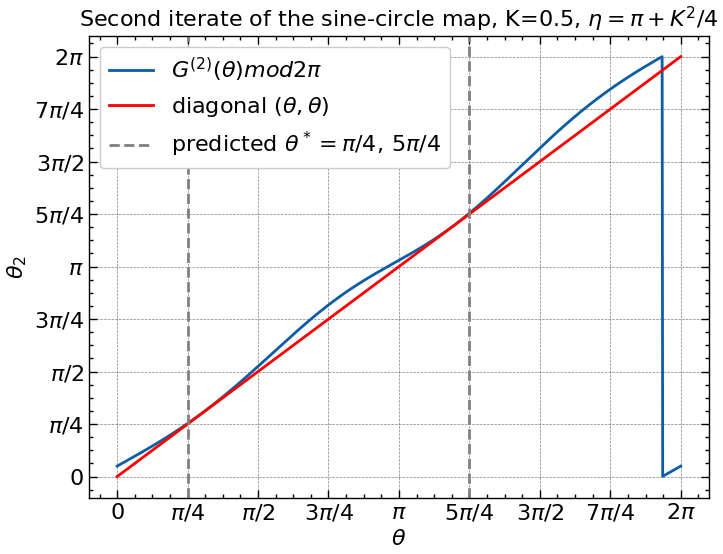
\includegraphics[width=0.75\textwidth]{Figure_3.png}
    \caption{Exact second iterate of the sine-circle map for \(K=0.5\).}
\end{figure}
\subsubsection{Replacing \(\sin\theta\) with \(\sin2\theta\)}
The first iterate is 
\begin{equation}
    \theta_1=\theta+\pi+\delta+K\sin2\theta
\end{equation}
and the second
\begin{equation}
    \theta_2=\theta+2\pi+2\delta+K\sin2\theta+K\sin\ins{2\theta+2\pi+2\delta+2K\sin2\theta}
\end{equation}
but to leading first order 
\begin{equation}
    \sin\ins{2\theta+2\pi+2\delta+2K\sin2\theta}\simeq\sin2\theta
\end{equation}
so 
\begin{equation}
    \theta_2\simeq\theta+2\pi+2\delta+2K\sin2\theta
\end{equation}
and the locking condition becomes 
\begin{equation}
    2\delta+2K\sin2\theta^*=0
\end{equation}
or 
\begin{equation}
    \sin2\theta^*=-\delta/K
\end{equation}
so 
\begin{equation}
    \abs{\delta}\leq\abs{K}
\end{equation}
giving the full width 
\begin{equation}
    2\abs{\delta}=2\abs{K}
\end{equation}
so it goes like K this time. The difference comes from the behavior under half a turn. When the angle is multiplied by 2, the half turns instead of contributing a negative contribution, they add up positively.